\section{背景}
本プロジェクトでは、「視覚や聴覚に頼れない状況で役立つ装置の開発」をコンセプトとし、障がい者が抱える問題を当事者目線で検討し、実用的な装置の開発に取り組んできた。頼れない感覚を別の手段で補うことで、不便を解消し、安全で快適な生活を支援することを目指している。
聴覚障がいや視覚障がい、色覚の障がい者を対象とした4つのグループに分かれ、それぞれ、特定の言葉や音に反応するデバイス、画像の色をユニバーサルデザインに変換するアプリ、自力で避難することが難しい人のための補助デバイス、障がい者が自然を楽しむためのデバイスの開発を行っている。

\section{課題の設定と到達目標}
\subsection{Group A: 色覚班}
色覚障がい者にとって見えにくい資料やグラフが社会に広く存在している。
この問題を解決するため、色覚障がい者が図やグラフを認識しやすくするアプリケーションを開発することを目指した。
本研究では、スマートフォンを用いて画像を撮影し、色変換を行う仕組みを構築した。

\subsection{Group B: 聴覚班}
高齢者や中途失聴者などの聴覚障がい者は、孤立しやすく、難聴であることを周囲に知られたくないという懸念を抱えている。
そこで、周囲に気づかれることなく、自身への呼びかけに気づけるよう補助し、孤立や不安を軽減するデバイスの開発を行う。

\subsection{Group C: 災害支援班}
視覚障がい者・聴覚障がい者などの、災害時に自力での避難が困難な避難行動要支援者が多数おり、避難時に置き去りなどの問題が発生している。
そこで、災害時において、避難行動要支援者が周囲の人々に助けを求めることを補助し、避難における自助・共助を行うことのできるデバイスの開発を目指す。

\subsection{Group D: 自然エンタメ班}
風の音や木々の揺れなど、日常的に自然の楽しさを体感している。
しかし、視覚や聴覚に障害のある方はそれが難しいと考えた。
自然を誰でも楽しめるようにしたい。
そこで、視覚や聴覚情報の相互変換を可能にするデバイスを開発し、障害の有無に関わらず誰でも自然を楽しめるようにし、自然の新たな楽しみ、価値をデザインする。

\section{課題解決のプロセスとその結果}
\subsection{Group A: 色覚班}
\subsubsection{対象ユーザーのニーズ分析}
岡部2002\cite{okabe2002color}を既存研究とし調査を行い、異なるタイプの色覚障がい(赤緑、青黄、全色盲)の特徴を整理。
さらに、オンラインアンケートを実施し、ユーザーのニーズを把握した。
\subsubsection{技術の選定}
PythonのOpenCVを用いて色変換アルゴリズムを実装し、PythonAnywhereでホスティングしてスマートフォンやPCからアクセス可能なウェブアプリケーションを構築した。
\subsubsection{ユーザーテストの実施}
色覚障がい者のボランティアによるテストを実施し、色の識別が容易になることで情報理解が向上したとのフィードバックを得た。
\subsubsection{成果物}
赤緑色覚障がい者においてはグラフや資料の情報認識が向上した。
一方で、青黄色覚障がいや全色盲への対応にはさらなる改良が必要であることが判明した。

\subsection{Group B: 聴覚班}

\subsection{Group C: 災害支援班}

\subsection{Group D: 自然エンタメ班}
目的を達成するために、RaspberryPiを用いたカメラ型デバイス「オトフォトン」を作成し、写真と音の相互変換を行う。
具体的には、撮った写真に応じた音楽を選曲し再生する機能と、録音した環境音を元にビジュアルアートを生成する機能を実装した。
また、デジタルデバイドを考慮し、誰でも扱いやすいデジタルカメラに寄せたデザインにした。

\begin{figure}[h]
  \centering
  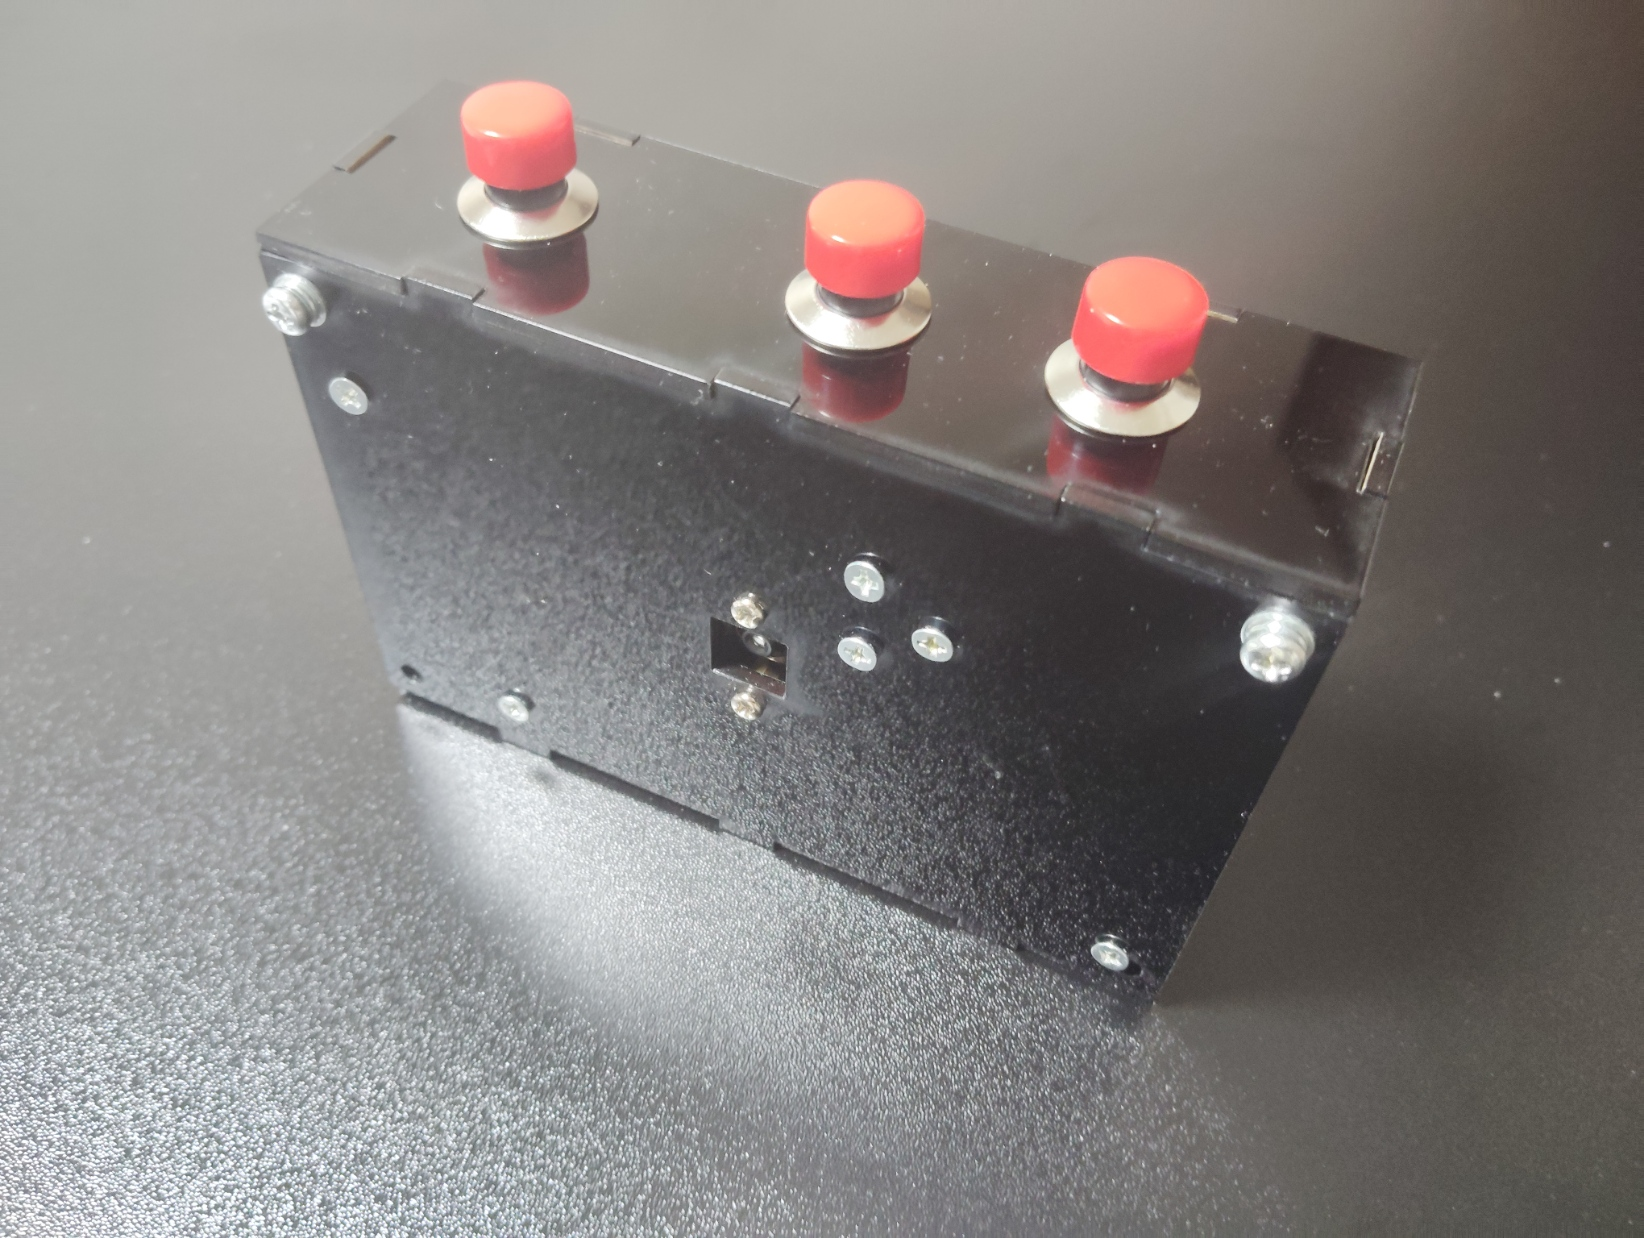
\includegraphics[width=0.45\textwidth]{pages/report/images/otophoton.jpg}
  \caption{オトフォトン}
  \label{fig:otophoton}
\end{figure}

\section{結論と展望}
\subsection{Group A: 色覚班}
本研究では、色覚障がい者が情報を正確に認識できる色変換アプリケーションを開発し、一定の成果を得た。
一方で、画像処理の遅さやUIの直感性の不足が課題として残った。
今後は以下の改善を図る。
\begin{itemize}
  \item 処理速度の向上
  \begin{itemize}
    \item アルゴリズムの最適化やクラウド処理の活用で、リアルタイム処理を可能にする。
  \end{itemize}
  \item UI/UXの改善
  \begin{itemize}
    \item 簡便で使いやすいデザインを採用し、視覚的フィードバック機能を充実させる。
  \end{itemize}
  \item アクセシビリティと多言語対応
  \begin{itemize}
    \item 多様なユーザーに配慮した機能と複数言語対応を進める。
  \end{itemize}
  \item 社会実装の推進
  \begin{itemize}
    \item 教育機関や企業での普及を目指し、色覚障がい者が情報を平等に享受できる社会の実現に寄与する。
  \end{itemize}
\end{itemize}
  本研究の成果を基にさらなる改良を重ね、色覚障がい者の生活や社会参加の向上に貢献していきたい。

\subsection{Group B: 聴覚班}

\subsection{Group C: 災害支援班}

\subsection{Group D: 自然エンタメ班}
音楽やビジュアルアートを好みに応じてカスタマイズできる機能等、細かな機能の追加をしたい。
また、このデバイスによって、自然の新たな楽しみ方を実現し、新しい価値をデザインしていきたい。
